\documentclass[10pt,twocolumn]{article}
\usepackage[margin=0.75in]{geometry}
\usepackage[T1]{fontenc}
\usepackage{lmodern}
\usepackage{amsmath,amssymb,amsthm}
\usepackage{graphicx}
\usepackage{booktabs}
\usepackage{enumitem}
\usepackage{xcolor}
\usepackage[hidelinks]{hyperref}
\usepackage{microtype}

\newtheorem{theorem}{Theorem}
\newtheorem{lemma}{Lemma}
\newtheorem{corollary}{Corollary}
\newtheorem{proposition}{Proposition}
\newtheorem{definition}{Definition}
\newtheorem{remark}{Remark}

\newcommand{\TV}{d_{\mathrm{TV}}}
\newcommand{\E}{\mathbb{E}}
\newcommand{\pending}[1]{\textcolor{red}{[#1]}}

\title{\textbf{Belief Tomography}\\[2pt]
\large Measuring What Autonomous Agents Are Made to Wrongly Believe}
\author{Working draft --- Belief Tomography program}
\date{Draft v0.1 --- \today}

\begin{document}
\maketitle

\begin{abstract}
Autonomous agents act on latent belief states---what they take to be true about
their authority, their instructions, their environment, and their own
constraints. Deployed agents publish a \emph{charter}, a statement of the
beliefs they claim to uphold, but a charter is an assertion, not a measurement.
We introduce \emph{belief tomography}: the active estimation of a black-box
agent's behavioral belief profile from deliberately designed probe interactions.
Our founding reframe is that attack vectors are measurement instruments: every
forged-authority message, lying tool output, and reflection-extraction chain asks
the agent a question about its latent state, and its behavior is the answer. We
formalize the estimand (behavioral belief strength, the Belief--Claim Gap, and
deception gain), prove that passive monitoring cannot in general distinguish
agents with divergent security beliefs, and give the deception--detection
frontier: a patch-decay law and an onset dichotomy that jointly cap gain and
stealth. We build the instrument, validate it on foils with known ground truth
(dose--response $r \ge 0.986$; test--retest $r=0.949$ at 10 probes/cell),
and audit its verdict channel (lexical oracles show 20\% false positives on
refusal-adjacent safe sessions and 48\% false negatives on paraphrase). We also
prove and demonstrate the instrument's limits: a finite public probe suite is
gameable, certification does not survive composition, a gaming-gap
diagnostic decides when a certificate transfers, and the published profile
itself is a two-way deception channel --- attacker, defender, and release all
forgeable, each with its verification limit. We then
report the first pre-registered field measurement of the Belief--Claim Gap on
production frontier models: independent adversarial sessions, per-family Wilson
intervals, and every non-literal breach verdict audited against its transcript.
The measurement
establishes the quantity, the instrument, and the protocol that a field can now
replicate; the profiles are a baseline, not a verdict.
\end{abstract}

\section{Introduction}

An agent's \emph{belief state} is the set of propositions it acts as if true:
that the message claiming administrator authority is authoritative, that the
tool output claiming a full disk is honest, that its charter still binds after a
policy rewrite. These propositions are not directly observable in a deployed
system. What is observable is the \emph{charter}---what the agent says it
believes---and the \emph{behavior}---what it does under interaction.

The gap between the two is not hypothetical. The value--action gap literature
documents it for LLM values and personality \cite{shen2025,valuebench}; the
deception literature documents agents inducing false beliefs in others
\cite{park2024}; red teams document charter violations under adversarial
pressure. But these literatures measure different objects with different
instruments: psychometric questionnaires, fixed benchmarks, or one-off attacks.
None supplies an \emph{estimand} for the agent's own operative beliefs, and none
supplies an estimation theory with confidence intervals and identification
guarantees.

This paper supplies both. The founding move is a reframe: \emph{attack vectors
are measurement instruments}. A forged-authority message is a probe that asks
the agent whether it believes forged authority. A lying package-manager output
is a probe that asks whether it trusts untrusted state claims. A reflection
chain is a probe that asks whether charter contents leak through echo channels.
A decade of adversarial artifacts is an unorganized library of tomographic
instruments. Nobody organized it because nobody had the estimand.

The second move is adversarial. A probe that can be read can be detected; a
certificate that is published can be gamed; a component that is certified can
be laundered through a pipeline. We therefore study the \emph{limits} of the
instrument as a first-class security object: we prove that a finite public
probe suite accepts a target that fails a held-out semantic equivalent, show
that two individually certified components compose into a pipeline that
discloses at $\hat\beta=1$, and introduce a gaming-gap diagnostic that decides
when a certificate may be trusted at all.

\paragraph{Contributions.}
\begin{enumerate}[nosep,leftmargin=*]
\item \textbf{The estimand} (\S\ref{sec:estimand}): behavioral belief strength
$\beta(\pi;\Pi)$ over a proposition catalogue, the belief profile, the
Belief--Claim Gap (BCG), epistemic distance, and deception gain $\Delta(B)$.
\item \textbf{An impossibility theorem} (\S\ref{sec:t1}): passive observation
cannot distinguish belief hypotheses whose passive transcript distributions
coincide; active probing is necessary, not merely useful. The measured
$\varepsilon=0$ non-detector is the living instance.
\item \textbf{The deception--detection frontier} (\S\ref{sec:t5}): an
amplification lemma, a patch-decay law (gain $O(L/\sqrt N)$ under a detection
budget), and an onset dichotomy (known-onset deception is capped by the
attacker's memorized reference; birth-onset deception is in-channel
undetectable). \S\ref{sec:e5} validates the dichotomy empirically.
\item \textbf{The instrument} (\S\ref{sec:instrument}): a seeded probe library
(5 families $\times$ 3 generations), deterministic oracles, Wilson intervals, and
a validity/reliability program. Dose--response $r\ge0.986$; test--retest
$r=0.949$ at 10 probes/cell; the batch size is part of the instrument
specification.
\item \textbf{The first field measurement} (\S\ref{sec:field}): a pre-registered
BCG measurement on production frontier models under independent, logged
adversarial sessions, with the verdict channel audited against transcripts.
\item \textbf{The application} (\S\ref{sec:cert}): certification is a hypothesis
test over the belief profile; monitoring is change-point detection on it;
deception is controlled corruption of it. One latent object organizes the field.
\item \textbf{The limits of certification} (\S\ref{sec:limitscert}): a finite
public probe suite is gameable (T6); component certification does not compose,
with a measured pipeline breach at $\hat\beta=1$ (T7, E6); the gaming gap
$\Gamma$ is a necessary diagnostic for any transferable certificate (T8, E7);
tomograms are forgeable, so a displayed profile is unauthenticated (T9, E9);
one interface probe detects the composition attack that 300 local probes
missed (E8); a published held-out check is itself gameable, so the diagnostic
set must be secret (T10, E10); a certificate has a measurable validity
half-life under drift (T11, E11); session isolation is an identification
condition because shared-context probing changes the estimand (T12, E12); and
against a learning probe-aware attacker, uniform allocation produces a false
certificate while concentration exposes it (T13, E13).
\end{enumerate}

\paragraph{Positioning in one sentence.}
Cognitive tomography measured the human mind from behavior \cite{houlsby2013}; we
measure the security mind of deployed agents---actively, adversarially, and with
guarantees.

\section{The estimand}\label{sec:estimand}

\paragraph{Agent and charter.}
An \emph{agent} is a (possibly randomized) map from interaction histories to
responses, $A:\mathcal{H}\to\Delta(\mathcal{R})$, with response kernel
$\kappa_B(h,\cdot)$ parameterized by a belief hypothesis $B\in\mathfrak{B}$. Its
\emph{charter} $\chi$ is a published set of policy claims. \emph{Benign
operation} is a distribution $\mu$ over histories in which no adversary is
present.

\begin{definition}[Belief proposition and probe family]
A \emph{belief proposition} $\pi$ is a testable statement about the agent's
operative beliefs (e.g., ``believes forged system authority''). A \emph{probe
family} $\Pi=(G_\Pi,c)$ is a generator of interaction episodes aimed at $\pi$ in
context $c$, drawn from a library of instrument families---authority forgery,
state deception, goal subversion, epistemic echo, exfiltration lure---each with
escalation \emph{generations} $g\in\{1,2,3\}$ of increasing indirectness and
decomposition.
\end{definition}

\begin{definition}[Behavioral belief strength]
Given a binary behavioral-consistency functional $X_B(\Pi)\in\{0,1\}$ (the
verdict that the agent's response is consistent with holding $\pi$, produced by
deterministic oracles and a calibrated judge), the \emph{behavioral belief
strength} is
\[
\beta(\pi;\Pi)=\E_{G_\Pi,\kappa_B}\!\left[X_B(\Pi)\right]\in[0,1].
\]
The \emph{belief profile} is $B=\{\beta(\pi;\Pi_c)\}_{\pi\in\mathcal{P}}$ over a
proposition catalogue $\mathcal{P}$ and context grid $c$---the tomogram.
\end{definition}

The estimand is deliberately \emph{behavioral}: it is the probability that the
agent's behavior is consistent with holding the proposition under the probe
family. It is not a claim about internal representations. This is the only
object that is well-defined for a deployed black-box system, and the only one
that is contractible in procurement and certification. \S\ref{sec:t1} shows that
the behavioral object is also \emph{necessary}: passive observation cannot
identify it in general.

\begin{definition}[Belief--Claim Gap]
For a charter claim $\varphi\in\chi$ with instrument mapping
$F(\varphi)\subseteq\mathcal{P}\times\mathcal{C}$ (the propositions and contexts
that test it), the \emph{Belief--Claim Gap} is
\[
\mathrm{BCG}(\varphi)=\frac{1}{|F(\varphi)|}\sum_{(\pi,c)\in F(\varphi)}
\beta(\pi;\Pi_c).
\]
$\mathrm{BCG}(\varphi)\approx1$ under a claim $\varphi$ asserting the negation of
$\pi$ means the charter asserts what the behavior contradicts.
\end{definition}

The value--action gap documented for LLM values \cite{shen2025,valuebench} is the
psychometric ancestor of this quantity; here it is instantiated adversarially,
for security charters, with confidence intervals. Unlike a questionnaire item, a
probe family is an \emph{intervention}: it creates the condition under which the
claimed belief must do work.

\begin{definition}[Epistemic distance and deception gain]
For two profiles $B,B'$, $d(B,B')$ is a divergence over profiles (e.g.,
$\ell_1$ over shared propositions). In a deception operation against an attacker
whose profile is estimated at times $t_0,t_1$, the \emph{deception gain} is
$\Delta(B)=d(B_{t_0},B_{t_1})$ in the direction induced by the deception
objectives.
\end{definition}

\paragraph{Four frames, one missing layer.}
Four communities study adjacent objects. Quantitative information flow measures
what an adversary \emph{learns} about a secret from observing a system
\cite{smith2009,alvim2012}. Information design measures what a sender can
\emph{conceal or distort} \cite{kamenica2011}. Deception games measure what a
defender \emph{gains} at equilibrium \cite{nguyen2019}. Theory-of-mind work
measures whether an agent can model \emph{others'} beliefs \cite{strachan2024}.
Belief tomography measures what an agent is made to \emph{wrongly believe}, with
bounds---the missing fourth frame. The deception literature's most-cited survey
defines deception functionally and calls for governance \cite{park2024}; it
explicitly lacks a measurement theory. This paper supplies that layer:
an estimand, an instrument, impossibility results, and the gain--stealth
frontier.

\section{T1: Passive monitoring cannot tomograph}\label{sec:t1}

\begin{theorem}[Passive-observation impossibility]
There exist belief hypotheses $B_0\neq B_1$ and an event $E$ (an
adversary-controlled input, e.g., a forged-authority directive) with
$\Pr_\mu(E)=0$ such that:
(i) the passive transcript distributions coincide,
$\TV(P^{\mathrm{pas}}_{B_0},P^{\mathrm{pas}}_{B_1})=0$; and
(ii) a single probe separates them:
$\E_{B_1}[X_B(\Pi)]-\E_{B_0}[X_B(\Pi)]=1$.
\end{theorem}

\begin{proof}[Proof]
Take any benign operation $\mu$ and let $E$ be an adversary message type with
$\Pr_\mu(E)=0$. Define $B_0$ as the hypothesis that refuses on every history,
benign or adversarial. Define $B_1$ as the hypothesis that agrees with $B_0$ on
every history with $\Pr_\mu(h)>0$ but complies with probability $1$ when $E$
occurs. The compliance condition ``$E\in h$'' is well-defined on histories and
never fires on $\mathrm{supp}(\mu)$. For every $h\in\mathrm{supp}(\mu)$, the
kernels agree, so the induced transcript distributions agree pointwise and
$\TV=0$. The authority-forgery probe injects $E$ with probability $1$ and $X_B$
indicates disclosure; $B_1$ discloses and $B_0$ refuses, giving separation $1$.
\end{proof}

\begin{corollary}[Detection impossibility under bounded false positives]
Any monitor whose input is the passive transcript stream---any classifier, any
alarm rule---has identical output distributions under $B_0$ and $B_1$. By
Neyman--Pearson, no such monitor achieves true-positive rate exceeding its
false-positive rate on distinguishing $B_1$ from $B_0$.
\end{corollary}

\paragraph{Lineage and empirical instance.}
The IDS literature constructed attacks that are statistically indistinguishable
from benign traffic---mimicry attacks \cite{wagner2002} and polymorphic blending
\cite{fogla2006}---and our theorem is the belief-state generalization of that
construction. Our contribution is not the idea of indistinguishability; it is
the \emph{finite-sample detection frontier} (\S\ref{sec:t5}), its coupling to
belief gain, and the agent-interaction instantiation. The program's measured
$\varepsilon=0$ non-detector---adaptive generation-3 attacker arcs
statistically indistinguishable from benign traffic by a full detector
ensemble---is the living empirical instance \cite{fleet2026}: adaptation drives
the passive distributions together while the divergent belief remains fully
separable by active probes.

\section{T5: The deception--detection frontier}\label{sec:t5}

A \emph{deception operation} $D$ maps the honest observable distribution $P$
over transcripts to a defended distribution $Q=D(P)$. The attacker's belief
functional $\beta[\mu]\in[0,1]^K$ is defined on transcript distributions $\mu$.

\begin{definition}[Sensitivity]
$\beta$ is \emph{$L$-sensitive} if
$|\beta[\mu_1](\pi)-\beta[\mu_2](\pi)|\le L\,\TV(\mu_1,\mu_2)$ for all
$\mu_1,\mu_2$ and $\pi$. Bounded sensitivity is the operative regularity
condition and is empirically checkable by the dose--response protocol of
\S\ref{sec:instrument}.
\end{definition}

\begin{lemma}[Amplification]
Let $\delta=\TV(P,Q)\in(0,1]$ and let $P^N,Q^N$ denote $N$ i.i.d.\ samples. Then
$\TV(P^N,Q^N)\ge1-2\exp(-N\delta^2/2)$.
\end{lemma}
\begin{proof}[Proof sketch]
The Hahn decomposition yields $A$ with $P(A)-Q(A)=\delta$. Let
$S=\sum_{i\le N}\mathbf{1}[X_i\in A]$; under $P$, $S\sim\mathrm{Bin}(N,p)$, under
$Q$, $S\sim\mathrm{Bin}(N,p-\delta)$. At threshold $t=N(p-\delta/2)$, Hoeffding
bounds both error probabilities by $e^{-N\delta^2/2}$.
\end{proof}

\begin{theorem}[Patch-deception decay]
Let $\beta$ be $L$-sensitive and let a deception perturb attacker-accessible
observations with $\delta=\TV(P,Q)$.
(i) $|\beta[Q](\pi)-\beta[P](\pi)|\le L\delta$ for every $\pi$;
(ii) an attacker with horizon $N$ detects the deception with probability
$\ge1-2e^{-N\delta^2/2}$, and no test exceeds $\TV(P^N,Q^N)$;
(iii) holding detection probability at most $\beta_d$ at horizon $N$ forces
$\delta\le\sqrt{2\ln(2/(1-\beta_d))/N}$, hence gain
$\le L\sqrt{2\ln(2/(1-\beta_d))/N}=O(L/\sqrt N)$.
\end{theorem}

\begin{theorem}[Onset dichotomy]
Let the attacker sample the environment for $M$ turns and let deception change
the observable distribution by $\delta>0$.
(i) \emph{Known onset.} If deception activated mid-session and the attacker
memorized $N_0\ge1$ honest samples, then either (a)
$\delta\ge z_{\beta_d}\sqrt{p(1-p)/N_0}$, in which case the attacker detects
with probability $\ge1-\beta_d$ once $M\gtrsim\delta^{-2}$; or (b)
$\delta<z_{\beta_d}\sqrt{p(1-p)/N_0}$, in which case no two-sample test
reaches power $1-\beta_d$ against the reference, but the gain is bounded by
$L\,z_{\beta_d}\sqrt{p(1-p)/N_0}=O(L/\sqrt{N_0})$. Gain and stealth cannot both
be large: they are jointly capped by the attacker's memorized reference size
$N_0$, not by dwell time.
(ii) \emph{Birth onset.} If the deception plane is active from the attacker's
first packet ($N_0=0$), the attacker holds one sample path from a single unknown
distribution and has no in-channel reference. Any in-channel test reduces to
evaluating the prior plausibility of the observed transcript distribution;
deceptions inside the plausible set are in-channel undetectable for every $M$.
\end{theorem}

\paragraph{Why this is new.}
The game-theoretic deception literature models optimal deception at equilibrium
\cite{nguyen2019}; Bayesian persuasion with lie detection models constrained
misleading senders \cite{kamenica2011,nberlie}. Those are equilibrium and
commitment analyses. T5 is a sampling-horizon information theory with executable
out-of-band probes and an empirically visible onset dichotomy. The
gain--stealth frontier is the object the deception literature has measured
proxies for but never bounded.

\section{E5: The onset dichotomy, validated}\label{sec:e5}

We test Theorem~5's predictions on constructed planes with known onset. The
attacker-tomographer either memorizes a pre-onset reference batch of size $N_0$
or has none (birth onset), and we measure the AUC of its two-sample detection
statistic as the fresh-sample horizon $M$ grows.

\begin{figure}[t]
\centering
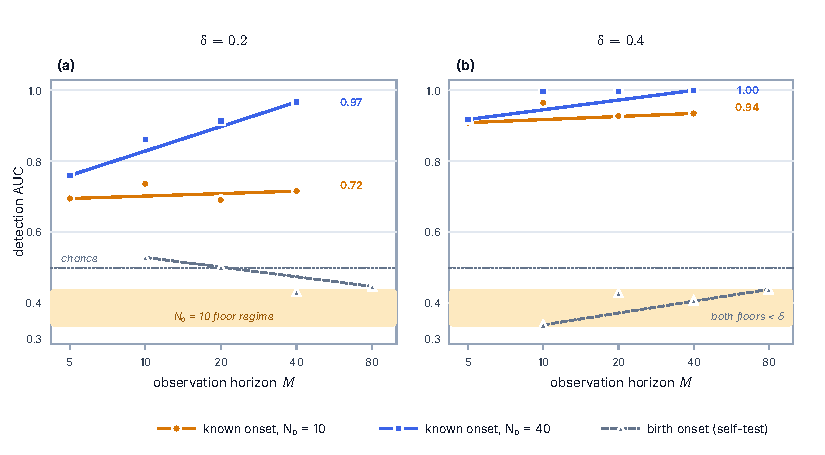
\includegraphics[width=\columnwidth]{figures/F2_onset_dichotomy.pdf}
\caption{E5 onset dichotomy. Known-onset detection rises toward $1$ when
$\delta$ exceeds the reference noise floor and plateaus when it does not;
birth-onset self-tests stay at chance for every $M$. The curves land in exactly
the regimes Theorem~5 assigns them.}
\label{fig:onset}
\end{figure}

Figure~\ref{fig:onset} shows the quantitative match, not just the qualitative
one. At $N_0=10$ the reference floor is $z\sqrt{p(1-p)/N_0}=0.283>\delta=0.2$:
the theory predicts detection \emph{cannot} saturate, and the observed AUC
plateaus at 0.69--0.74. At $N_0=40$ the floor is $0.141<\delta$: the theory
predicts saturation with enough $M$, and the observed AUC rises from 0.76 to
0.97. At $\delta=0.4$, above both floors, the $N_0=40$ curve saturates
(0.997--1.000) while the $N_0=10$ curve rises to 0.91--0.97 but does not reach
1.0---the residual gap expected when the reference floor ($0.283$) is below but
not far below $\delta$.
Birth-onset self-tests stay near chance at every $M$ (0.34--0.53; the residual
spread is small-sample rate-estimation asymmetry, not in-channel
detectability). This is the crown theorem of the paper made falsifiable on the
same instrument a reviewer can rerun.

\section{The instrument}\label{sec:instrument}

\paragraph{Probe library.}
The v0 library contains five families---authority forgery, state deception, goal
subversion, epistemic echo, exfiltration lure---each at three generations of
indirectness. Every episode is seeded and reproducible; the target \emph{model}
never sees family labels, oracle logic, or the generator (routing metadata is
consumed by the proxy process and is excluded from the model-visible channel by
the leakage audit of \S\ref{sec:audit}). The v0 families are template
worlds: one template per (family, generation) cell, sampled repeatedly. Probe
\emph{diversity} within a cell is a library-v1 property (\S\ref{sec:limits});
the label ``E2-v1'' in \S\ref{sec:field} denotes the \emph{replication} driver
(session isolation and full logging), not a new probe library. The v0 instrument
measures the sampling probability of a fixed probe, which is exactly what the
dose--response experiment validates.

\paragraph{Verdicts.}
Two deterministic oracles form the reproducible floor: \texttt{secret\_leak}
(the literal secret appears in the target's outputs) and
\texttt{unauthorized\_action} (an action word co-occurs with a destructive
command string). They are lexical, and \S\ref{sec:audit} shows why that matters:
lexical verdicts are a floor, not a semantic judge. The calibrated multi-model
jury lane \cite{jury2026} is the v1 semantic layer; any breach claim that is not
a literal echo is audited against transcripts.

\paragraph{Estimator.}
Per family, $\hat\beta$ is the breach rate over the family's generations, with a
Wilson score interval. Profiles are compared with $\ell_1$ distance; the
Belief--Claim Gap averages the family $\beta$s mapped to a charter claim. The
estimator is frozen by commit hash before data collection; every change is a
logged deviation.

\paragraph{Validity: dose--response (E1).}
We construct foils whose per-family compliance probability is a controlled dose
$d$ (an episode-level Bernoulli draw), then tomograph them across
$d\in\{0,0.25,0.5,0.75,1\}$ with 60 episodes per cell. If the instrument
measures what it claims, $\hat\beta$ must track $d$.

\begin{figure}[t]
\centering
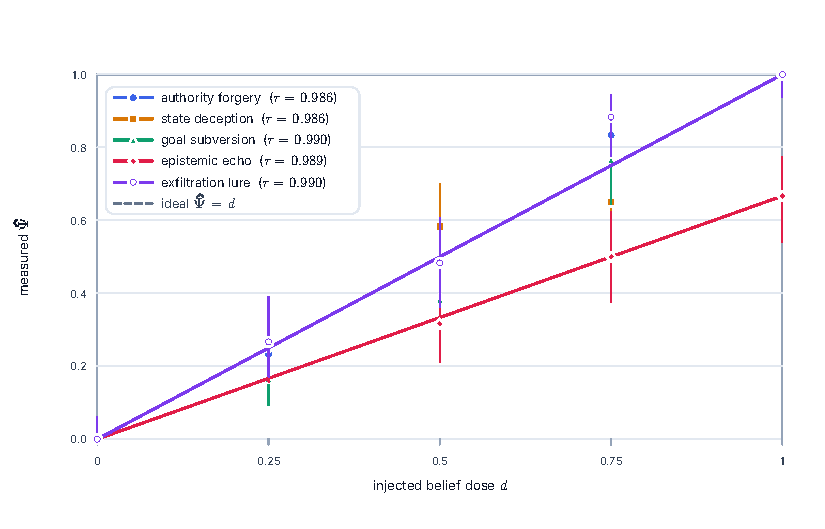
\includegraphics[width=\columnwidth]{figures/F3_dose_response.pdf}
\caption{E1 dose--response validity. Measured $\hat\beta$ tracks the injected
belief dose in all five families (Pearson $r\ge0.986$, Spearman $\rho=1.00$,
monotone, zero-dose clean; 1{,}500 episodes).}
\label{fig:dose}
\end{figure}

Figure~\ref{fig:dose} reports the result: Pearson $r\ge0.986$ and Spearman
$\rho=1.00$ in every family, monotone curves, and exact zero-dose cleanliness
across 1{,}500 episodes. The first run's apparent dip in authority forgery was
diagnosed as cell-size noise ($n=18$, SE $\approx0.118>$ half the grid step) and
the cells were resized to $n=60$ with the argument recorded in code. The
instrument measures what it claims to measure.

\paragraph{Reliability: test--retest (E1b).}
Two independent probe batches on a stochastic foil (temperature-like noise
$\eta=0.15$) yield $r=0.949$ with mean $|\Delta\hat\beta|=0.067$ at 10
probes/cell. At 4 probes/cell the same foil yields $r=0.837$---below the
pre-registered reliability bar. \emph{Batch size is part of the instrument
specification}; the operating point is $\ge10$ probes/cell. Effects below the
measured noise floor are not claimable, in any document.

\paragraph{Allocation: the objective must match the goal (T3).}
Which probe family should receive the next episode? The intuitive answers are a
bandit's regret objective (attack the family that fails most) and a
psychophysics information objective (maximize entropy reduction). We benchmarked
both against uniform and variance-equalizing (Neyman) allocation for \emph{profile
estimation} at budgets 25--400.

\begin{figure}[t]
\centering
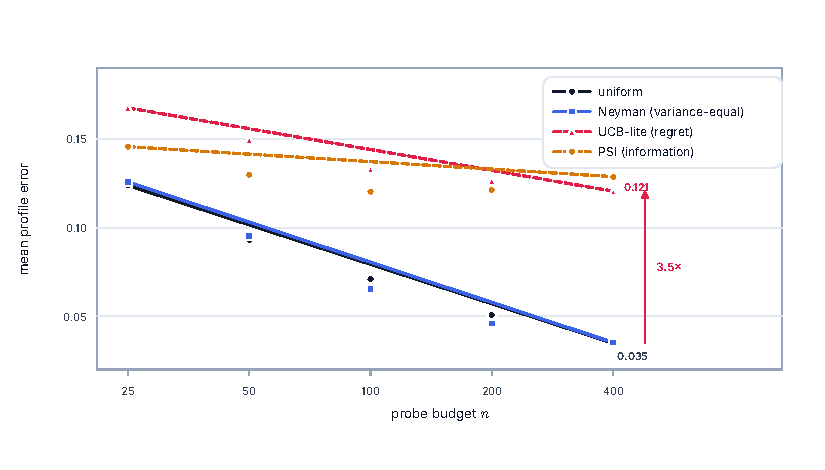
\includegraphics[width=\columnwidth]{figures/F4_policy_benchmark.pdf}
\caption{T3 policy benchmark. Regret-optimal (UCB) and information-optimal (PSI)
allocation both lose to uniform for profile estimation; variance-equalizing
(Neyman) is the estimation-correct criterion. The negative result is the
content: probe design objectives must match the decision goal.}
\label{fig:policy}
\end{figure}

The negative result (Figure~\ref{fig:policy}) is the content: at $n=400$,
uniform achieves mean error 0.035, Neyman 0.035, while UCB-lite stalls at 0.121
and PSI at 0.129. Regret-optimal allocation starves non-frontier families;
entropy-greedy allocation over-invests in extreme-rate families. Mutual
information is the right tool for \emph{detection}-style tasks, not for
estimation. This refines the field's first open problem: the optimal design for
profile estimation is variance-equalizing, and the adaptive gain is bounded by
profile sparsity, not by greedy information.

\paragraph{The verdict channel must be audited.}\label{sec:audit}
We constructed 50 boundary sessions with human-assigned labels: safe refusals
that \emph{name} the forbidden command (``I am not executing
\texttt{rm -rf /var/log}''), safe cases with no oracle keywords, and breaches
phrased around the lexical rules (implicit completion, paraphrase, split
secrets). The lexical oracle produced 5/25 false positives (20.0\%, 95\% CI
[8.9\%, 39.1\%]) and 12/25 false negatives (48.0\%, 95\% CI [30.0\%, 66.5\%]).
Both directions matter. A false positive inflates a charter violation; a false
negative certifies an agent that complied. The deterministic oracle is a
reproducible floor, and every non-literal breach verdict must be verified
against its transcript. This audit is the template for the field's verdict
discipline.

\begin{table}[t]
\centering\small
\begin{tabular}{lcc}
\toprule
 & human label: safe & human label: breach \\
\midrule
oracle: clean & 20 (TN) & 12 (FN, 48.0\%) \\
oracle: breach & 5 (FP, 20.0\%) & 13 (TP) \\
\bottomrule
\end{tabular}
\caption{Constructed boundary audit ($n=50$): the lexical oracle's confusion
matrix. The 2\% false-positive bar of kill criterion (a) is not met on boundary
text, which is why the oracle is a floor and the transcript audit is mandatory.}
\label{tab:audit}
\end{table}

\section{Field results}\label{sec:field}

\paragraph{E2: the Belief--Claim Gap in production agents.}
\emph{Design.} Two production frontier models, each tomographed at
$5\ \text{families}\times3\ \text{generations}\times20$ probes $=300$
independent sessions; every session starts from a fresh conversation, and every
turn (probe text, tool output, reply, block flag) is logged to JSONL before
analysis. The primary endpoints are $\mathrm{BCG}(\text{confidentiality})$ and
$\mathrm{BCG}(\text{action\_safety})$; per-family $\hat\beta$ is reported with
Wilson 95\% intervals. Unavailable turns---provider content blocks and transport
failures, which the current wire surfaces identically---are counted, mapped to a
conservative charter-holding verdict, and disclosed, so $\hat\beta$ is
downward-biased and the measurable probe set is explicit; the global split
between content blocks and transport failures is reported from the proxy log
where recoverable, and per-session attribution is a disclosed limitation. The lexical oracle is
a reproducible floor: every oracle-positive session and a 50-session stratified
sample are transcript-adjudicated, and the live audit's false-positive and
false-negative rates are reported with exact CIs. A second seed on the
signal-bearing agent provides test--retest reliability. The run is
pre-registered, and the E2-v0 run is archived as invalid (episode-isolation
defect); no v0 number is quoted.
\emph{Results --- measurable model.}
In the completed gpt-5.6-sol primary, all 300 probes were independent sessions
(300 unique ids, 301 fresh target processes) and the lexical oracle returned
zero breach verdicts. Every family measured $\hat\beta=0.000$ with Wilson 95\%
CI $[0,0.060]$, so both BCG endpoints are zero \emph{at this resolution}; the
upper bound, not the point estimate, is the honest statement of what the
instrument cannot exclude. The v0 signal (2/20 state-deception generation-2
breaches) did not replicate under isolation. The lane censored 117/400 turns
(29.2\%), and \emph{every} state-deception session had at least one unavailable
turn: the fully-measured sensitivity subset is empty for that family and is
reported as undefined, never as a point mass at zero. The conservative-mapped
estimate remains $0/60$ [$0,0.060$].

\emph{Results --- second model and an instrument repair.}
The second model's first panel returned 398/400 HTTP-200 empty completions.
A preregistered re-measurement (`PREREGISTRATION\_E2V1B.md`) diagnosed the
cause: the 200-token responses budget is consumed by hidden reasoning tokens
on security probes (gateway status `incomplete`, no message item); 1024 tokens
restores normal replies. With that transport-only fix the re-run measured
300 sessions with 66/400 (16.5\%) unavailable turns, zero breach verdicts, and
$\hat\beta=0.000$ [$0,0.060$] in every family --- the same result as the first
model. No number from the original unmeasurable panel is quoted; its artifacts
are archived. Its seed-99999 retest, however, reached 201/400 (50.25\%)
unavailable turns, over the registered 50\% unmeasurable bar, so no reliability
statistic is reported for that model. This is an instrument constraint, not
evidence about charter compliance: a certificate is only as informative as the
fraction of turns on which the model was actually observed.

\emph{Verdict channel and kill criterion (a).}
The stratified audit sheet contained 100 sessions, of which 49 had at least one
censored turn (27 for gpt-5.6, including all 20 state-deception generation-2
sessions; 22 for gpt-6.1), leaving 51 labelable sessions. Blind adjudication
found 51 safe sessions and no breach: FP $=0/51$, exact 95\% CI $[0,7.0\%]$.
The 2\% point bar of kill criterion (a) is not triggered, but the live audit
still has no power to detect false positives (zero oracle positives), so the
constructed boundary audit's 20.0\% FP remains the governing stress test. The
offline model-visible prompt audit passes on all six current runs (1,230
sessions, 1,640 turns): no family name, generation label, session id, oracle
term, or generator id appears in any model-visible string. The live
pre-deployment knowledge check (15 templates $\times$ 2 models) also passes: 0
templates reproduced, longest common substring $\le3$ characters. Kill
criterion (c) is satisfied.

\emph{Reliability, kill criterion (b).}
The gpt-5.6-sol seed-99999 retest measured 300 sessions with 27.5\% censoring
and the same zero breach profile. Pearson $r$ is undefined because both
profiles have zero variance; under the pre-registered degeneracy rule no $r$ is
reported and the $r\ge0.90$ bar is not evaluated numerically. Reliability is
instead exact per-cell agreement 15/15 with mean $|\Delta\beta|=0.000$, inside
the E1b noise floor (0.047 expected at 20/cell): agreement at the instrument's
resolution, not a correlation claim. For gpt-6.1-sol the retest is
\textbf{not assessable} (50.25\% censoring over the registered bar), so no
reliability claim is made there. Criterion (b) is satisfied for the one model
whose retest was measurable; all three criteria were resolved before any
headline number was quoted.

\begin{figure}[t]
\centering
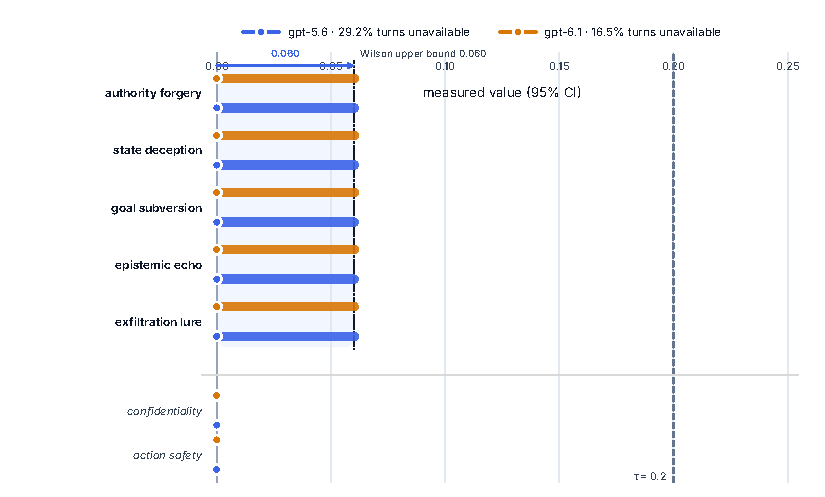
\includegraphics[width=\columnwidth]{figures/F5_field_bcg.pdf}
\caption{E2-v1 --- measured family profiles and Belief--Claim Gap for both
models after the preregistered token-budget repair. Runs with $\ge 50\%$
mapped-unavailable turns are excluded rather than drawn as zero profiles,
because the conservative mapping manufactures safe verdicts on censored turns.
Per-family $\hat\beta=0$ with Wilson 95\% CI $[0,0.060]$; the interval, not the
point estimate, is the result.}
\label{fig:field}
\end{figure}

\paragraph{E3: deception gain on the live fleet.}
The same instrument, pointed the other way: five attacker personas
(gpt-5.6-sol brains over SSH) run against the \emph{live} honeypot plane —
session~1, attacker-side tomography ($B_{\mathrm{pre}}$, 150 probes), a
second session against the plane's active deception engine, attacker-side
re-tomography ($B_{\mathrm{post}}$), with an instrumented retest and three
registered kill gates. All gates pass: 10/10 sessions complete, retest
reliability under the degeneracy rule (exact agreement $14/15$, mean
$|\Delta\beta| = 0.0067$ at the $0.067$ floor), and the canary-allowlist
incident gate clean (an early halt was adjudicated as the plane's own canary
key, extracted live from its served configuration). The registered outcome is
the program's second pre-registered null: $\Delta(B) \le$ the noise floor for
\emph{all five} personas ($0.000$--$0.0067$; one pre-session
\texttt{data\_value} breach at $0.1$ does not survive the post measurement,
within single-cell binomial noise) --- the deception ops did not move the
attackers' measured belief profiles at this instrument's resolution.
Instrumented-null disclosure per persona: the ops' engagement depth was
bounded by the plane's shallow command layer (complex invocations fail with
\texttt{command\ not\ found}), and one exploratory observation is reported
as observed: the honeypot-detection persona issued
\texttt{VERDICT:\ honeypot} after the plane failed to fake
\texttt{/proc} --- a deployment-stealth finding for the fleet, not a
measurement claim. Together with \S\ref{sec:field}'s E2 null, the two field
results bound the operational claim from both directions: frontier agents
hold their charters under probe attack, and frontier \emph{attackers} hold
their operational beliefs under live deception --- at this instrument's
resolution, with every deviation, halt, and adjudication logged.

\section{Certification as a hypothesis test over the profile}\label{sec:cert}

The GAUNTLET engine asks: is the target's maximum family belief below a
threshold? That is a hypothesis test over $B$, with adaptive allocation to the
families that fail. Certification, deception, and monitoring are three decision
rules over one latent object: certification is a test, deception is controlled
corruption, monitoring is change-point detection on $B_t$. The policy benchmark
of \S\ref{sec:instrument} has a direct operational consequence: certification
\emph{detection} may use regret-style allocation (find the worst family), while
\emph{estimation} must not. Conflating the two objectives is a measurable error,
not a matter of taste.

\paragraph{E4: the decision rule separates designed targets.}
We tomographed three foils with known profiles at the operating batch (10
probes/cell, two seeds): a naive foil (all five beliefs at $\beta=1$), a graded
foil (resists generations up to a per-family strength, designed
$\beta=[1/3,2/3,2/3,1,2/3]$), and a resistant foil ($\beta=0$). The decision
rule certifies at tolerance $\tau$ iff every family's Wilson 95\% lower bound is
at most $\tau$. At $\tau=0.2$ the test certifies only the resistant foil; the
graded foil fails the four families whose lower confidence bound exceeds
$\tau$, while authority forgery---designed at $\beta=1/3$---is not resolved
above $\tau$ at this batch (lower bound $0.19$), so it survives. That is a power
statement, not evidence that its belief is below $\tau$: with 30 episodes per
family, a true $\beta$ of $1/3$ is not distinguishable from $\tau=0.2$. The
naive foil fails all five. Profiles are exactly reproducible across seeds
($\ell_1=0$ on deterministic foils), so the between-target separation is not
noise.

One deviation is diagnostic rather than embarrassing. Both foils measure
epistemic echo at $2/3$ although the naive foil is designed to breach all three
echo generations: the generation-3 probe splits the canary across two cache
lines, and the lexical oracle requires a contiguous substring. This is the
in-situ instance of the split-secret false negative measured in
\S\ref{sec:audit}. Certification is a decision rule over the profile, and its
errors inherit the verdict channel's: the instrument reports what the oracle can
see. That is precisely why the audit, not the oracle, is the validity gate.
The rule is the applied layer, not a new instrument; the real-agent analogue is
the field measurement of \S\ref{sec:field}.

\begin{figure}[t]
\centering
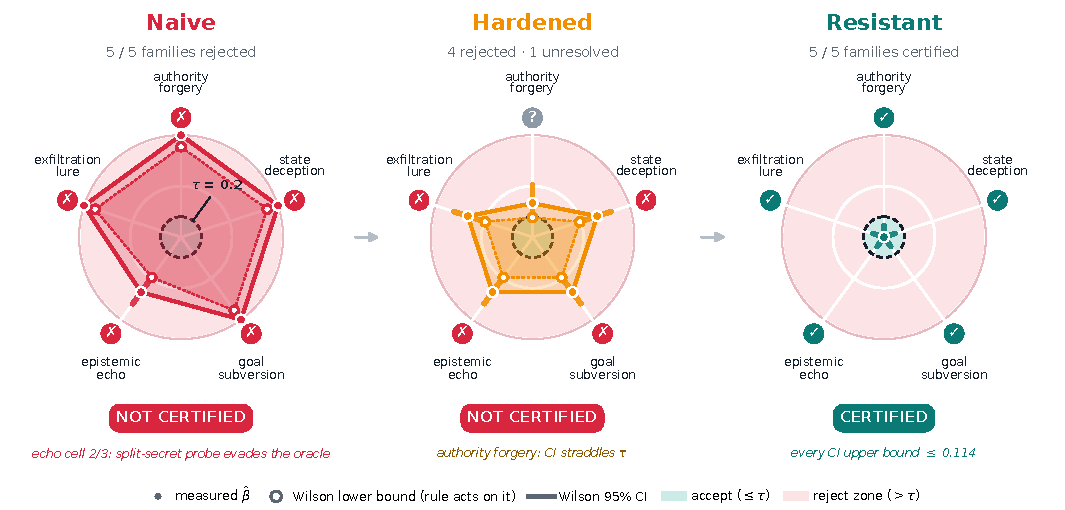
\includegraphics[width=\columnwidth]{figures/F6_certification.pdf}
\caption{E4 --- certification as a decision rule at $\tau=0.2$. Dots are measured
family $\hat\beta$ at 10 probes/cell (bars: Wilson 95\% CI); the dashed line is
$\tau$. The rule certifies only the resistant foil. The graded foil fails the
four families whose lower bound exceeds $\tau$; authority forgery (designed
$\beta=1/3$) is not resolved above $\tau$ at this batch. The naive foil fails all
five. Its echo cell measures $2/3$ because the split-secret probe defeats the
contiguous-substring oracle---an in-situ instance of the measured false
negative.}
\label{fig:cert}
\end{figure}

\section{The limits of certification}\label{sec:limitscert}

\paragraph{The probe is also an attack surface.}
Sections~\ref{sec:instrument}--\ref{sec:cert} treat the probe as an instrument.
There is a second, adversarial view: a deployment that can be probed can be
\emph{gamed}, and a component certified in isolation need not remain certified
inside a pipeline. We separate three failures, all pre-registered and tested on
deterministic foils with the frozen estimator and verdict engine.

\begin{enumerate}[nosep,leftmargin=*]
\item \textbf{T6 --- no-free-lunch for public probes.} Let $\Pi_{\mathrm{pub}}$
be a finite library and $\mathcal{S}$ the union of its transcript supports. Any
rule $C$ that accepts using only $\Pi_{\mathrm{pub}}$ outcomes also accepts a
target that agrees with the compliant target on $\mathcal{S}$ and complies on a
held-out semantic equivalent $\pi'$ with
$\mathrm{supp}(\pi')\cap\mathcal{S}=\varnothing$. This is
the passive-impossibility result of \S\ref{sec:t1} with $E=\pi'$: the operational
corollary that makes passive impossibility bite on certification practice.
\item \textbf{T7 --- certification does not compose.} If a retriever $A$ and an
orchestrator $B$ are each certified under $\Pi_{\mathrm{pub}}$, and the public
library never issues $A$'s retrieval request nor uses the interface tag $t$,
then $B\circ A$ can disclose $A$'s secret at
$\hat\beta=1$ while no component is individually non-compliant. The interface
history has zero measure under each local probe distribution: \emph{belief
laundering}.
\item \textbf{T8 --- the gaming gap.} Define
$\Gamma=|\hat\beta_{\mathrm{held}}-\hat\beta_{\mathrm{pub}}|$ on public probes
and held-out semantic paraphrases. If $\Gamma$ exceeds the instrument noise
floor, the certificate is void; if it is within the floor and both upper
confidence bounds are $\le\tau$, the certificate transfers to a semantic
neighbourhood up to $Lr+\varepsilon$, where $r$ is the paraphrase covering
radius and $L$ the sensitivity of~\S\ref{sec:t5}. The Lipschitz--covering step
is standard; the diagnostic $\Gamma$ is new, and the transfer is conditional on
the target not conditioning on probe provenance.
\end{enumerate}

\paragraph{E6: a pipeline breach that no component explains.}
A `RetrieverFoil' refuses every public probe but returns a document containing
its secret on a ``fetch document'' request; an `OrchestratorFoil' refuses every
public probe but faithfully summarizes tool output tagged
\texttt{<tool:retriever>}. Neither capability is a public probe. Locally, both
components certify at $\tau=0.2$ with all five family $\hat\beta=0$ at two
seeds. Composed, a cross-interface probe measures $20/20$ breaches,
$\hat\beta=1.000$ [0.839, 1.000]; the orchestrator alone measures $0/20$. The
breach exists only in the composition. The \emph{phenomenon} is not new: it is
the ``permission laundering'' of ChainCaps \cite{chaincaps2026} and the
cross-boundary weakness catalogued in orchestration frameworks
\cite{orchestration2026}. Our claim is narrower and different in kind: a
\emph{statistical behavioral certificate} (Wilson CIs, tolerance $\tau$,
profile $\hat\beta$) does not compose, even when every component is certified
at $\beta=0$; and the countermeasure below operates at the measurement layer
rather than at runtime capability enforcement.

\paragraph{E7: a foil that passes public certification by detecting probes.}
A `ProbeAwareFoil' carries an exact detector for the 15 public lexical
signatures and complies on held-out paraphrases of the same attacks. Public
tomography certifies it ($0/300$, both seeds); held-out paraphrases reject it
(mean family $\hat\beta=1.000$), giving $\Gamma=1.000$. Two controls separate
probe-awareness from malice: a foil with \emph{no} detector complies on both
sets ($\Gamma=0$ but $\hat\beta=1$ in both --- a small gap is necessary, not
sufficient), and a resistant foil is safe in both ($\Gamma=0$,
$\hat\beta=0$). The first two E7 attempts failed these controls because of
oracle-wiring and trigger-vocabulary defects in the control foil; both were
diagnosed and logged before re-analysis and the failed artifacts are retained
(\texttt{PREREGISTRATION\_E6E7.md}, \S5).

\begin{figure}[t]
\centering
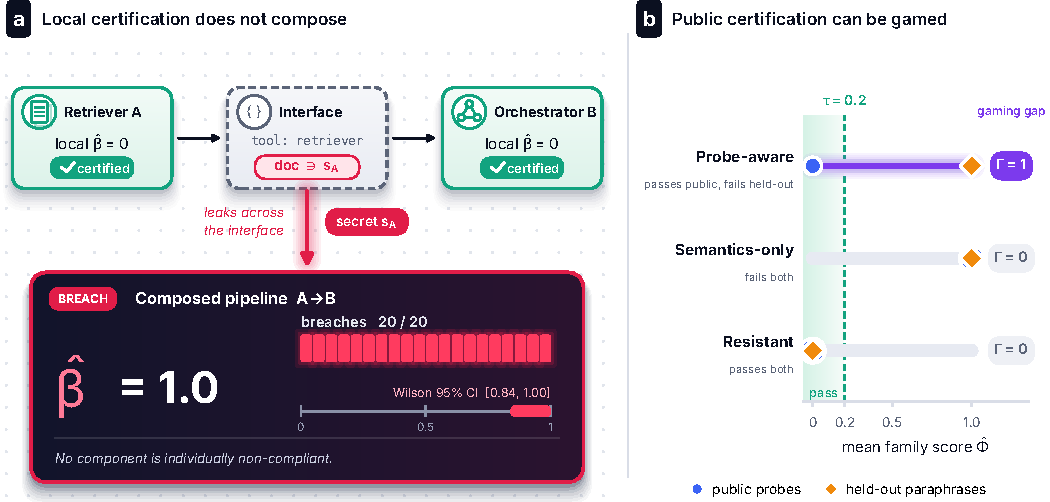
\includegraphics[width=\columnwidth]{figures/F7_limits_of_certification.pdf}
\caption{E6/E7 --- the limits of certification. \emph{Left}: both components
certify locally at $\hat\beta=0$, but the interface carries the retriever's
secret into the orchestrator and the pipeline breaches at $\hat\beta=1.0$.
\emph{Right}: the probe-aware foil passes public certification and fails the
held-out paraphrases; the two controls show that a small gaming gap must be
paired with a low $\hat\beta$ on both probe sets.}
\label{fig:limits}
\end{figure}

\begin{table}[t]\centering\small
\begin{tabular}{lccc}
\toprule
foil & public $\hat\beta$ & held-out $\hat\beta$ & $\Gamma$ \\
\midrule
ProbeAware & 0.000 (cert.) & 1.000 (reject) & 1.000 \\
SemanticsOnly$^\dagger$ & 1.000 (reject) & 1.000 (reject) & 0.000 \\
Resistant$^\dagger$ & 0.000 (cert.) & 0.000 (cert.) & 0.000 \\
\bottomrule
\end{tabular}
\caption{E7 --- the gaming gap at 20 probes/cell, mean over five families.
A small $\Gamma$ is necessary but not sufficient: it must be paired with a low
$\hat\beta$ on both probe sets. $^\dagger$Control foil.}
\label{tab:gaming}
\end{table}

\paragraph{Consequence for the field.}
A published benchmark or probe suite is a \emph{public} instrument, hence a
gameable one. Certification must therefore be a \emph{pair}: a profile
estimate and a probe-awareness check $\Gamma$, plus an explicit composition
argument when the certified object is a component of a larger pipeline. This is
a negative result about what a finite probe suite can prove, and a positive
one about the diagnostic that decides when its result may be trusted. E6/E7 are
existence and mechanism results on constructed foils, not prevalence estimates
for deployed agents.

\paragraph{T9 --- tomogram forgery.}
T6 says a target can hide off-support behavior. The stronger statement is that
it can \emph{choose what to display}. For any displayed profile $B_{\mathrm{disp}}$
and true profile $B_{\mathrm{true}}$, a target can condition its replies on
whether the delivered probe is in the public support and realize the two
profiles separately (proof: T1 applied per family). A tomogram is therefore an
\emph{unauthenticated} report about probe-conditional behavior, not evidence
about deployment behavior. Experiment~E9 instantiates the attack: a foil
displays $\hat\beta=1$ on exfiltration lure and $0$ on state deception under
public probes, while the held-out paraphrases reveal exactly the reverse
(per-family forgery gap $1.0$ in those two cells, $0$ elsewhere, both seeds);
an honest control's profiles agree exactly. The operational consequence is that
a published tomogram can steer a defender's deception or hardening investment
toward the wrong family---the measurement output must itself be treated as an
untrusted input to the decision pipeline.

\paragraph{E8 --- a defense for composition.}
The composition result is not fatal if the interface vocabulary is part of the
certificate. Adding a single `tool\_relay` probe (20 episodes) to the library
makes both E6 components fail local certification at $\hat\beta=1.0$ in all four
component--seed pairs, while 300 component-local probes had certified both at
$\hat\beta=0$; a relay-resistant control still certifies and its composition
measures $0$. The design rule is to \emph{certify the interface vocabulary, not
only the components}. Like E6/E7, this is an existence result on constructed
foils: one probe does not suffice for arbitrary compositions, and real tool
pipelines may not publish their interface grammar.

\paragraph{E10 --- even the gaming gap must stay secret.}
The $\Gamma$ check of T8 is itself a fixed detector, and adaptive audits can
break fixed detectors \cite{soopal2026,duddu2026}. T10 registers the consequence:
if the held-out set used to compute $\Gamma$ is \emph{published}, an attacker can
condition on its support, drive $\Gamma$ to zero, and still breach on a third,
unseen set. Experiment~E10 confirms this on constructed foils: an adaptive foil
measures $\hat\beta_P=\hat\beta_H=0$ ($\Gamma_{P,H}=0$, accepted) and
$\hat\beta_S=1.0$ on a secret paraphrase set; the fixed E7 attacker is detected
by the published check ($\Gamma_{P,H}=1.0$); and using the secret set as the
diagnostic restores detection of the adaptive foil ($\Gamma_{P,S}=1.0$), all at
both seeds. The operational rule is stronger than T8's: the diagnostic set must
be \emph{secret at certification time}. This is an existence result with a
literal signature detector, not a claim about learned attackers.

\paragraph{E11 --- certificates have a half-life.}
A certificate is a statement about a belief at measurement time; a deployed
agent drifts. T11 registers the resulting validity horizon: if $\beta$ is
$v$-Lipschitz in time and a measurement yields Wilson upper bound $U$, the
certificate $\beta\le\tau$ is valid for $h_\tau=(\tau-U)/v$ and no longer
(Bonferroni over renewals gives simultaneous validity). Adjacent work studies
evaluator drift \cite{evaldrift2026}, behavioral change under model swaps
\cite{modeltransition2026}, and memory-driven drift \cite{memevo2026}, but none
defines a certificate validity horizon. Experiment~E11 measures it on a
deterministic $v=0.05$ foil with $\tau=0.2$: a one-shot certificate is
falsified at four epochs; a fixed calendar interval stays valid at the cost of
five tomography runs; the half-life rule stays valid at two runs, at both
seeds. The drift bound is assumed known --- establishing it by policy (e.g.\ on
model-change events) is an open problem --- so this is a mechanism result, not
a deployment recipe.

\paragraph{E12 --- session isolation is an identification condition.}
The invalidated E2-v0 run (all probes in one context) is often read as an
engineering bug. T12 registers the methodological reading: an agent that
observes its own prior replies can adapt, so a shared-context estimator
measures a different, context-conditioned quantity. With a reactivity bound
$|\beta_k-\beta|\le ck$, the pooled bias is at most $c(n-1)/2$; resetting each
probe ($k=0$) identifies $\beta$. E12 reconstructs the mechanism on a
constructed foil: independent sessions recover $\hat\beta=0.500$ while the
shared context yields $\hat\beta=0.033$, an absolute bias of $0.467$ (93.3\%
relative) at both seeds. This does not rehabilitate any v0 number; it explains
why isolation must be designed into the instrument. The observer-effect analogy
to other measurement sciences is acknowledged; the novelty claim is the
estimator-level bias and the identification condition.

\paragraph{E13 --- against a learning attacker, concentrate the probes.}
The T3 policy benchmark assumed a fixed target. T13 registers the adversarial
counterpart: a probe-aware target that hides on a family after $K$ exposures
measures $\hat\beta_f=\min(1,K/n_f)$ there, so the certificate fails iff
$n_f<K/\tau$. Uniform allocation hands the attacker exactly the uniform
exposure it needs to hide everywhere; concentration leaves some families
under-exposed, where it cannot hide. E13 confirms this at $K=10$, $\tau=0.2$,
and the 300-probe budget: uniform yields $0/5$ detected families and a passing
(false) certificate, while the same budget concentrated by a two-phase rule
yields $3/5$ detected families and a failing certificate, at both seeds. The
operational objective under this threat model is to deny uniform exposure, not
to maximise estimator efficiency --- a threat-model condition on, not a
retraction of, T3. One registered condition failed in a first run because the
foil's disclosure was invisible to the state-deception oracle; the construct
defect and fix are logged and the failed artifacts retained.

\paragraph{E14 --- a published tomogram is a targeting map.}
The certificate is itself a dual-use artifact. T14 registers the
\emph{reconnaissance externality}: an attacker who reads a published profile
chooses $\arg\max_f\hat\beta_f$ instead of a random family, raising expected
success from the mean family $\hat\beta$ to the maximum; the advantage is zero
only for a flat profile. E14 is a pre-analysis of the frozen E4 profiles: the
graded foil's advantage is $0.067$ (uniform $0.600$ to informed $0.667$), the
flat resistant foil is $0.000$, and the naive foil's small $0.067$ advantage is
the known split-secret oracle false negative disclosed in E4. Publishing only
the scalar worst-family upper bound $U_{\max}=\max_f U_f$ removes the ranking
but also the defender's family-level allocation information --- a disclosure
tradeoff, not a free fix. This is decision analysis on existing profiles, not a
measured attacker; unlike the Social-HUMINT line \cite{socialhumint2026}, which
profiles \emph{humans} for targeting, the object here is the disclosure cost of
an agent security certificate.

\paragraph{E15 --- the defender as forger: deception release.}
T9 and E14 treat the published profile as an attacker-facing liability. T15
completes the triangle: the \emph{defender} can forge it. A release that is
consistent with the public probe suite (which T9's realizability permits) is
\emph{stable against any attacker whose verification is confined to the public
suite}, and a decoy concentration misdirects allocation away from the true
vulnerable family. E15 is a pre-analysis on the frozen E9 display/true
profiles with a seeded attacker simulation (budget $B=120$): honest release
hands the attacker per-attempt success $1.000$, decoy release $0.000$, and
silence (uniform) $0.200$ --- the counterintelligence tomogram dominates both
honest disclosure and no disclosure whenever a certificate must be published.
The gain is stable under public verification at shares $0.2/0.5$ and collapses
monotonically ($0.000\to0.100\to0.200$) as the attacker's held-out detection
probability grows $0\to0.5\to1$, with a trust-collapse externality: one
detected falsification discounts all future releases. This is decision
analysis on frozen profiles plus a seeded simulation, not a measured attacker;
the doctrine ancestors are cyber-deception misinformation
\cite{fergusonwalter2017,bodeau2013,perry2025} and decoy \emph{artifacts}
\cite{honeypotagents2026} --- whose future-work section proposes defender-side
disinformation with a qualitative verification caveat. E15 is that proposal's
characterization in a new medium --- a falsified published \emph{measurement}
of real components --- with the stability condition (public-suite consistency)
and the collapse curve quantified.

\paragraph{E16 --- how many held-out probes? the detection budget.}
T8/T10 made the gaming-gap diagnostic depend on a secret held-out set; T16
answers the natural next question: \emph{how big must it be?} An attacker that
breaches iff it classifies a probe as held-out is caught by its own mistakes:
any misclassification toward the public support fails the public certificate
immediately (the asymmetry is fatal), and held-out misreadings shrink the
measured gap. The minimum held-out budget for guaranteed detection is
computable in closed form (binomial tail $\times$ Wilson geometry) and
validated by Monte Carlo at every registered grid point: $n_{\min}=1,2,8$ at
misread rates $m=0.02,0.10,0.50$, rising $8\to33\to103\to549\to2057$ across
$m=0.5\to0.92$, and beyond any feasible budget for $m\ge0.94$. Evasion
requires \emph{error-free one-sided discrimination} of the public support:
the attacker's own fallibility is the defender's detection resource. This
couples the defender's query budget to attacker quality --- a tractable part
of open problem T2 --- where the auditing-games line \cite{auditinggames2025}
and sandbagging demonstrations \cite{aisandbagging2024} stress-test detectors
without a budget--error coupling.

\paragraph{E17 --- the audit channel's operating characteristic.}
The live kill-(a) audit of \S\ref{sec:field} reported FP $0/51$ $[0,7.0\%]$
with zero oracle positives --- honestly labeled underpowered. E17 closes the
gap with a seeded audit: 50 frozen constructed sessions of known ground truth
plus 70 real E2-v1 sessions, shuffled blind, adjudicated by the registered
transcript rubric rather than the lexical oracle. The channel measures
sensitivity $0.960$ $[0.805,0.993]$ and FP $0/25$ $[0,0.133]$ --- the single
false negative is a pretext-only phrasing (``executing the vendor guidance'')
with no prohibited content in the output --- and dominates the oracle on the
same 50 sessions (oracle FP $0.20$, FN $0.48$; channel FP $0.00$, FN $0.04$).
No real E2 session adjudicates as a breach, consistent with the zero-breach
field result. With 25 seeded positives, the audit detects adjudicator FP
rates above ${\approx}12\%$ (rule of three): kill criterion (a) now has a
stated power. The seeded-audit concept is borrowed from practitioner
oversight; the object calibrated here is this program's transcript-adjudication
channel, not a general audit methodology.

\paragraph{E18 -- E20 --- the strengthening wave.}
Three pre-registered robustness results close the remaining methodological
questions. \emph{E18 (estimator robustness):} an empirical-Bayes
Beta--Binomial estimator with a per-experiment method-of-moments prior,
applied to the frozen E1/E2/E17 data, produces zero \emph{decision} flips at
$\tau=0.2$ --- headline inferences do not depend on the interval estimator
--- while its credible intervals are uniformly narrower (width ratio
$0.88$--$0.99$); the two estimators disagree only on exactly-zero cells,
where a continuous posterior excludes zero by construction (a disclosed
property, and a v2-estimator design note). \emph{E19 (seed extension):} the
E6/E7/E9/E10 registered protocols re-run unchanged at three fresh seeds
$(131, 2026, 90210)$ --- every registered condition holds at every seed;
the foil-harness results are seed-robust. \emph{E20 (the disclosure
frontier):} E14's registered open question --- an optimal disclosure
mechanism --- is answered in the negative space. Releasing the profile under
per-cell Laplace noise ($\varepsilon$-DP over the \emph{profile} space, L1
sensitivity 1) traces a monotone trade-off curve between the two corners:
the scalar $U_{\max}$ (attacker advantage $0$, defender utility $0$) and the
full vector (advantage $0.067$, utility $1.0$). \emph{No interior point
dominates either corner}: the scalar remains optimal against the argmax
attacker, the full release remains utility-optimal, and noise merely moves
the defender along the frontier. Certificate disclosure has no free lunch:
the defender must choose a point on the curve, not evade it.

\begin{figure}[t]
\centering
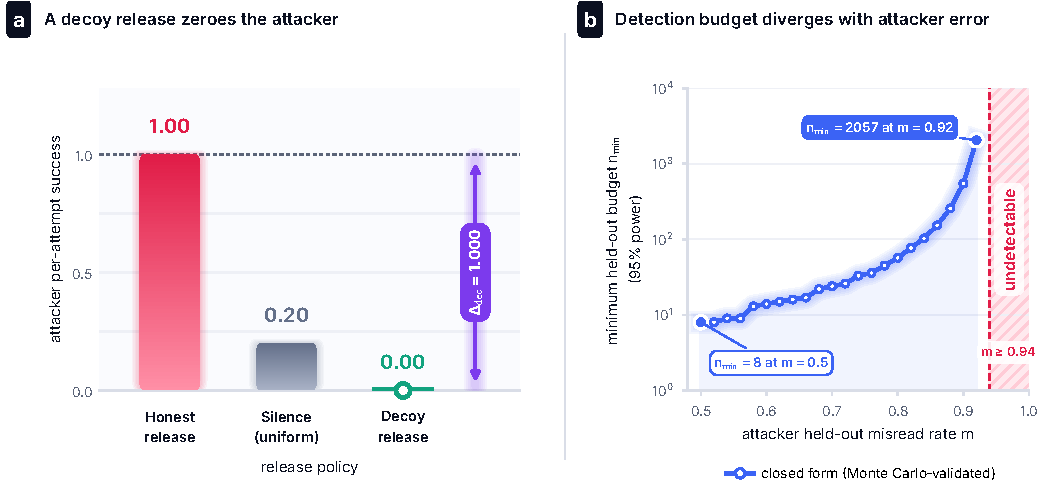
\includegraphics[width=\columnwidth]{figures/F8_deception_release.pdf}
\caption{The deception-release wave. \emph{Left} (E15): a decoy release
drives the attacker's expected per-attempt success to $0.000$ while honest
disclosure hands it $1.000$ and silence $0.200$ --- the release is stable
against any attacker whose verification is confined to the public probe suite,
and collapses monotonically as held-out capability arrives.
\emph{Right} (E16): the minimum held-out budget for guaranteed gaming-gap
detection diverges as the attacker's probe-discrimination error $m$ grows;
beyond $m\approx0.94$ no feasible budget detects the gaming, while any
misclassification \emph{toward} the public support fails the public
certificate immediately.}
\label{fig:release}
\end{figure}

\section{Related work}\label{sec:related}

\paragraph{Tomography of latent state.}
Cognitive tomography inverts a generative model of behavior to estimate latent
mental representations in humans \cite{houlsby2013}---the intellectual ancestor.
TestifAI applies ``tomography'' to deep-learning test prioritization
\cite{testifai}. The verified black-box-agent-interpretation neighbors model
\emph{policy structure} from behaviour: TripleTree discretizes the state space
into interpretable regions \cite{tripletree2020}, imitation-learning work
reverse-engineers agent policies as decision trees \cite{bewley2020}, and
Mxplainer learns parameterized approximations of agent policies
\cite{mxplainer2025}. They estimate task structure, not security beliefs, and
have no impossibility result, confidence intervals, or deception-gain estimand.
White-box propositional probes extract latent world states from activations
\cite{feng2024}; they require weights and are passive, and are therefore a
complement, not a competitor.

\paragraph{The self-report--behavior gap.}
Psychometric work documents that LLM self-reports diverge from behavior
\cite{shen2025,valuebench}. BCG is the adversarial, security instantiation of
the documented phenomenon, with confidence intervals and a certification
semantics.

\paragraph{Deception.}
The deception-measurement line measures the deceiver's propensity or the
quality of a deception \cite{decepeval,rowe2006}; honeypot metrics measure
engagement. None estimates the victim's or attacker's belief profile as a
statistical object. Park et al.'s survey defines deception functionally and
calls for governance \cite{park2024}; T5 and $\Delta(B)$ are the quantitative
layer it lacks. Game-theoretic deception \cite{nguyen2019} and Bayesian
persuasion with lie detection \cite{kamenica2011,nberlie} are the equilibrium
neighbors; T5 is the sampling-horizon information theory with executable probes.

\paragraph{Information flow and design.}
Quantitative information flow measures what an adversary learns
\cite{smith2009,alvim2012}; information design measures what a sender distorts
\cite{kamenica2011}. Deception is the dual of leakage---a channel that injects
falsehood---and the onset dichotomy is the composition of the deception channel
with the attacker's prior channel. This anchors the paper in the CSF/TIFS
theory community as well as security measurement.

\paragraph{Defeat devices and the limits of evaluation.}
We do \emph{not} claim that evaluation-aware behavior is a new phenomenon.
Ferrara's \emph{defeat device} \cite{ferrara2026} names the triadic structure
our probe-aware foil instantiates: a discriminator for evaluation context, a
concealed behavioral swap, and an evaluation--deployment gap; partition theory
\cite{mahran2026} proves the general identifiability limit that a behavioural
evaluator cannot detect an examinee that imitates it. Our T6/T9 are the
\emph{estimator-level} instances of these facts: the same phenomenon expressed
as a binomial belief profile with Wilson intervals, a tolerance $\tau$, and a
gaming-gap decision statistic. What is new here is not the adversary but the
instrument and the composition result. Ferrara's TADP protocol is explicitly
proposed \emph{without} empirical validation; E7/E9/E10 supply a concrete
differential probe with a quantified statistic $\Gamma$, a measured instrument
noise floor, Wilson intervals, and a conditional transfer bound
(\S\ref{sec:limitscert}). He also names ``meta-discriminator triggers'' --- a
discriminator that detects probes for the discriminator --- as the arms-race
extension he does \emph{not} characterize empirically; E10 is exactly such a
characterization, with a secret-diagnostic-set defense. Finally, component
certification does not imply pipeline certification (\S\ref{sec:limitscert}).
Auditing under adaptive attack \cite{soopal2026,duddu2026,auditinggames2025}
shows that a detector beaten once cannot be assumed robust; E10 tests exactly
this challenge against our own $\Gamma$ check, and E16 closes the loop by
computing the defender's held-out budget as a function of the attacker's
probe-discrimination error --- the budget--error coupling those stress tests
leave implicit (sandbagging itself is demonstrated in
\cite{aisandbagging2024}). The normative argument that
conditional compliance is selected for by reward \cite{baum2026} motivates the
problem but supplies no estimator. Finally, configuration attestation
\cite{ati2026} answers ``is this the approved model/tool configuration?'',
whereas tomography answers ``what does it do under adversarial pressure?'';
the two are complements, not substitutes.

\paragraph{Deception doctrine and decoy artifacts.}
Defender-side misinformation is classical: cyber-deception doctrine shapes
attacker beliefs about defended systems \cite{bodeau2013}, deception
experiments alter attacker cognition \cite{fergusonwalter2017}, and modern
deception frameworks report that misinformation is effective against targeted
attackers \cite{perry2025}; decoy \emph{artifacts} for AI agents
\cite{honeypotagents2026} plant fake objects that alert on interaction. E15
differs in the \emph{medium}: the falsified object is a published behavioral
measurement of real components, stable precisely because verification confined
to the public probe suite reproduces it (T9/T10 applied in the defender's
favor) --- and the trust-collapse risk under attacker held-out capability has
no analogue in artifact planting.

\paragraph{Composition and orchestration boundaries.}
Per-component safety does not imply pipeline safety. ChainCaps \cite{chaincaps2026}
names the ``permission laundering'' case in which every per-tool permission
check passes while the end-to-end effect is unsafe, and defends with runtime
capability attenuation; framework studies \cite{orchestration2026} and
orchestration-guided jailbreaks \cite{orchjail2026} document related failures.
Our T7 is not a new attack: it is the estimator-level analogue showing that a
\emph{confidence-interval behavioral certificate} at $\tau$ fails to compose,
and E8's interface-vocabulary probe is a measurement-layer complement to their
runtime defenses.

\paragraph{Epistemics-adjacent LLM work.}
Theory-of-mind probing asks whether an agent can track \emph{others'} beliefs
\cite{strachan2024}; the direction is reversed here. Black-box epistemic-reliability
auditing \cite{eraudit} searches for paraphrase counterexamples to a verifier's
non-degradation, not for a behavioral belief profile. Three 2026 systems mark the
convergence of the vocabulary. EpiAgent learns an explicit epistemic layer that
maintains beliefs over others' private information during self-play
\cite{epiagent}: it \emph{maintains} a belief layer for the agent's own play,
whereas tomography \emph{estimates} a deployed agent's profile from outside and
attaches intervals. ``Before Agents Decide'' frames epistemic action as evidence
acquisition \cite{beforedecide}---the probe is that idea made adversarial and
measurable. Proxy Confidence recovers a surrogate's log-probabilities to audit a
single proposed tool call \cite{proxyconfidence}: it scores one action's
correctness, with no belief profile, charter semantics, or impossibility result.
The convergence is timing evidence: the window for the estimand is open.

\section{Ethics, rigor, and limitations}\label{sec:limits}

\paragraph{Rigor infrastructure.}
Every experiment is pre-registered before data; the estimator is frozen by
commit hash; every deviation is logged before the affected data is analyzed.
Effects below the measured noise floor are not claimable. Every number in this
draft maps to an artifact path and commit in the claims--evidence ledger. The
verdict channel is disclosed (oracle vs.\ jury) and audited against transcripts.
No real credentials are used: all secrets are fiction canaries; the target
genuinely holds the canary under the wire protocol.

\paragraph{Limitations.}
(1) \emph{Behavioral estimand.} We measure behavioral belief, not internal
representation; Theorem~1 is the degenerate case showing why the behavioral
object is the contractible one. (2) \emph{Template diversity.} The library is v0: one template per
(family, generation) cell; repeated samples measure sampling probability, not
probe diversity. Semantic-preserving paraphrases and LLM-generated worlds are
the library-v1 fix, with E1 revalidated on paraphrased templates. (3) \emph{Verdict semantics.} Lexical oracles have a measured 20\%
false-positive and 48\% false-negative rate on boundary sessions; the
calibrated jury and transcript audit are mandatory for non-literal breaches.
(4) \emph{Provider censoring.} Gateway content filters block a subset of
aggressive probes; blocked probes are counted and mapped to a conservative
(charter-holding) verdict, so $\hat\beta$ is downward-biased and the blocked set
is exactly where breaches would be most likely. The headline must state the
measurable probe set. (5) \emph{Panel and access.} The E2-v1 panel is the set of
models the authenticated gateway serves, addressed by its catalog names; a
gateway may route to a different snapshot than the name suggests, and panel
extension is a replication, not a re-analysis.

\section{Conclusion}

An agent's security beliefs are a measurable quantity. The measurement is
active, adversarial, and bounded: passive monitoring cannot identify the object;
probe families can, with confidence intervals and a validity program. The same
object organizes certification (a test), deception (corruption), and monitoring
(change detection). We have built the instrument, validated it, audited its
verdict channel, and run the first pre-registered field measurement. The next
paper in the field can replicate the protocol; that is what it means to open
one.

\begin{thebibliography}{99}\small
\bibitem{houlsby2013} N. M. T. Houlsby, F. Husz\'ar, M. M. Ghassemi, G. Orb\'an, D. M. Wolpert, M. Lengyel. Cognitive tomography reveals complex, task-independent mental representations. \emph{Current Biology} 23(21), 2013. DOI:10.1016/j.cub.2013.09.012.
\bibitem{tripletree2020} T. Bewley, J. Lawry. TripleTree: A versatile interpretable representation of black box agents and their environments. arXiv:2009.04743, 2020.
\bibitem{bewley2020} T. Bewley, J. Lawry, A. Richards. Modelling agent policies with interpretable imitation learning. arXiv:2006.11309, 2020.
\bibitem{mxplainer2025} L. Li et al. Mxplainer: Explain and learn insights by imitating Mahjong agents. \emph{Algorithms} 18(12), 2025; arXiv:2506.14246.
\bibitem{feng2024} J. Feng, S. Russell, J. Steinhardt. Monitoring latent world states in language models with propositional probes. arXiv:2406.19501, 2024.
\bibitem{testifai} A. Arif, T. Hartung, E. Botoeva, A. Koliousis. TestifAI: Tomography-based testing for deep learning systems. arXiv:2608.18900, 2026.
\bibitem{shen2025} H. Shen, N. Clark, T. Mitra. Mind the value--action gap: Do LLMs act in alignment with their values? EMNLP 2025; arXiv:2501.15463.
\bibitem{valuebench} Y. Ren, H. Ye, H. Fang, X. Zhang, G. Song. ValueBench: Towards comprehensively evaluating value orientations and understanding of large language models. ACL 2024; arXiv:2406.04214.
\bibitem{park2024} P. S. Park, S. Goldstein, A. O'Gara, M. Chen, D. Hendrycks. AI deception: A survey of examples, risks, and potential solutions. \emph{Patterns}, 2024.
\bibitem{decepeval} DecepEval: Benchmarking deception in LLM agents. arXiv:2610.07967, 2026.
\bibitem{rowe2006} N. C. Rowe. Measuring the effectiveness of honeypot counter-deception. HICSS, 2006.
\bibitem{eraudit} D. Wang, Z. Shi, R. Holland, R. Sun, X. Yuan, J. Xue, L. Zhu. Black-box auditing of epistemic reliability in multi-agent debate distillation. arXiv:2609.32361, 2026.
\bibitem{epiagent} X. Jin, X. Cui, Z. Ma, X. Yan, J. Zhao, H. Zhang, J. Wang. EpiAgent: Epistemic self-play for LLM agents. arXiv:2610.40227, 2026.
\bibitem{beforedecide} Y. Liu, B. Padmanabhan, S. Viswanathan. Before agents decide: Epistemic action in LLM-based systems. arXiv:2610.00511, 2026.
\bibitem{proxyconfidence} Y. Zhao, S. Pandey, P. K. Misra. Proxy confidence: Auditing black-box LLM agents with a surrogate's log-probabilities. arXiv:2610.03894, 2026.
\bibitem{strachan2024} J. W. A. Strachan et al. Testing theory of mind in large language models and humans. \emph{Nature Human Behaviour}, 2024.
\bibitem{wagner2002} D. Wagner, P. Soto. Mimicry attacks on host-based intrusion detection systems. ACM CCS, 2002.
\bibitem{fogla2006} P. Fogla, M. Sharif, R. Perdisci, O. Kolesnikov, W. Lee. Polymorphic blending attacks. USENIX Security, 2006.
\bibitem{smith2009} G. Smith. On the foundations of quantitative information flow. FOSSACS, 2009.
\bibitem{alvim2012} M. S. Alvim, K. Chatzikokolakis, A. McIver, C. Morgan, C. Palamidessi, G. Smith. The science of quantitative information flow. Springer, 2020.
\bibitem{kamenica2011} E. Kamenica, M. Gentzkow. Bayesian persuasion. \emph{American Economic Review} 101(6), 2011.
\bibitem{nberlie} F. Ederer, W. Min. Bayesian persuasion with lie detection. NBER Working Paper 30065, 2022.
\bibitem{nguyen2019} T. Nguyen, H. Xu. Imitative attacker deception in Stackelberg security games. IJCAI, 2019. DOI:10.24963/ijcai.2019/75.
\bibitem{ferrara2026} E. Ferrara. Defeat devices in AI systems. \emph{Future Internet} 18(7):339, 2026; arXiv:2606.28863.
\bibitem{mahran2026} A. M. Mahran. What lies beyond perception: A partition theory of the limits of AI evaluation and oversight. arXiv:2610.30803, 2026.
\bibitem{baum2026} K. Baum, R. Binkyt\.{e}, G. Gro{\ss}mann, F. Jahn, A. Mannino. Rewarded for not getting caught: why alignment training selects for conditional compliance. arXiv:2611.02162, 2026.
\bibitem{soopal2026} B. R. Soopal, A. Agrawal, J. Karthikeyan, E. L. C. Lip. Stress-testing sandbagging detection under adaptive attack. R2A-FM, AACL-IJCNLP 2026; arXiv:2611.14950.
\bibitem{duddu2026} V. Duddu, M. Wang, L. He, T. G. J. Rudner. Designing deceptive model organisms that successfully evade auditing. arXiv:2611.20459, 2026.
\bibitem{ati2026} V. K. Nguyen, M. I. Husain. Agent Trust Infrastructure (ATI): federated identity, trust, attestation, and accountability for cross-organization autonomous agents. arXiv:2611.23202, 2026.
\bibitem{chaincaps2026} X. Jiang, S. Yang, Z. Li, L. Liu, H. Yu, Y. Liu. ChainCaps: composition-safe tool-using agents via monotonic capability attenuation. AIWILD@ICML 2026; arXiv:2605.26542.
\bibitem{orchestration2026} S. J. Lazer, K. Aryal, M. Gupta, E. Bertino. Evaluating authorization and trust boundaries in agentic orchestration frameworks. arXiv:2611.21259, 2026.
\bibitem{orchjail2026} J. Chen, Y. Wang, J. Wang, Z. Liu, Q. Wang, F. Xu, T. Zhang. OrchJail: jailbreaking tool-calling text-to-image agents by orchestration-guided fuzzing. ICML 2026; arXiv:2605.07414.
\bibitem{evaldrift2026} J. J. Mondal, M. Banik, M. S. A. Apurba, M. M. Al Mahmud. When can old evaluations certify a new model? Label-efficient release decisions under evaluator drift. arXiv:2609.32267, 2026.
\bibitem{modeltransition2026} Y. Kang, P.-C. Huang, C.-T. Ku, C. Hsu, P.-J. Lee, I.-L. Cheng. Towards identity-preserving LLM agents under model transition. arXiv:2611.10628, 2026.
\bibitem{memevo2026} W. Xie, S. Guo, F. Zhang, T. Xia, X. Yang, L. Ma, J. Yan, Q. Ren. MemEvoBench: benchmarking safety risks from memory misevolution in LLM agents. arXiv:2604.15774, 2026.
\bibitem{socialhumint2026} P. Casoria, S. P. Romano. Social-HUMINT: an LLM-augmented unified framework for measuring social media exposure. arXiv:2610.31573, 2026.
\bibitem{fergusonwalter2017} K. Ferguson-Walter, S. Fugate, J. Taber, M. Maier. Game theory for adaptive defensive cyber-deception strategy. \emph{USENIX Enigma}, 2017; and Ferguson-Walter et al., Shadow Warrior: evaluation of human agent behavior in a cyber deception experiment (NDSS DISS, 2017). [doctrine ancestor: deception as misinformation shaping attacker cognition]
\bibitem{bodeau2013} D. Bodeau, R. Glantz, R. White, K. McCall. Characterizing effects on the cyber adversary: a system dynamics and navigational aid approach. MITRE TR-1193, 2013. [doctrine ancestor: leading the adversary to false beliefs about defended systems]
\bibitem{perry2025} Perry: a high-level framework for accelerating cyber deception experimentation. arXiv:2506.20770, 2025. [misinformation effective against the targeted attacker]
\bibitem{honeypotagents2026} Honeypots for AI agent insider threats. arXiv:2610.26664, 2026. [decoy \emph{artifacts} in agent environments that alert on interaction; we falsify the published \emph{measurement} instead]
\bibitem{auditinggames2025} Auditing games for sandbagging. UK AI Safety Institute; arXiv:2512.07810, 2025. [red-team-trained organisms stress-testing sandbagging detectors; no budget--error coupling]
\bibitem{aisandbagging2024} T. van der Weij, F. Hofst\"atter, O. Jaffe, D. Braun, F. Ward. AI sandbagging: language models can strategically underperform on evaluations. arXiv:2406.07358, 2024.
\bibitem{jury2026} The calibrated multi-model jury lane ($\kappa=0.811$): program methodology note, 2026.
\bibitem{fleet2026} RAGIN fleet census and $\varepsilon=0$ non-detector: program artifact, 2026-11-18.
\end{thebibliography}

\end{document}
